\section{Durchführung}
\subsection{Aufbau}
Der Aufbau des Versuchs ist in Abb.\ref{aufbau} dargestellt.  Er besteht aus einer Rubidiumdampflampe, dessen Licht durch eine Linse fokussiert wird und danach durch einen Filter auf die D$_1$-Komponente reduziert wird. Das D$_1$-Licht wird danach durch einen Polarisationsfilter und ein $\lambda/4$-Plättchen zirkularpolarisiert. Daraufhin durchquert es eine Zelle, welche mit Rubidium gefüllt ist und wird danach durch eine weitere Linse fokussiert und mit einer Photodiode detektiert. Die Rubidiumzelle wird extern geheizt um Rubidiumdampf zu erzeugen. Umgeben wird die Zelle von drei Helmholtzspulenpaaren. Eines wird in der Vertikalen genutzt, um das Erdmagnetfeld abzuschirmen. Die beiden anderen sind horizontal montiert, wobei eines davon zur Erzeugung des RF-Feldes dient. Die Signale von Photodiode und die Feldstärken können durch ein Oszilloskop aufgezeichnet werden. Zur Verhinderung von Störungen durch die Umwelt wird der Aufbau abgedeckt. Die Steuerung des RF-Feldes erlaubt es verschiedene Feldstärken im Sweep-Modus zu überstreichen.
\begin{figure}
  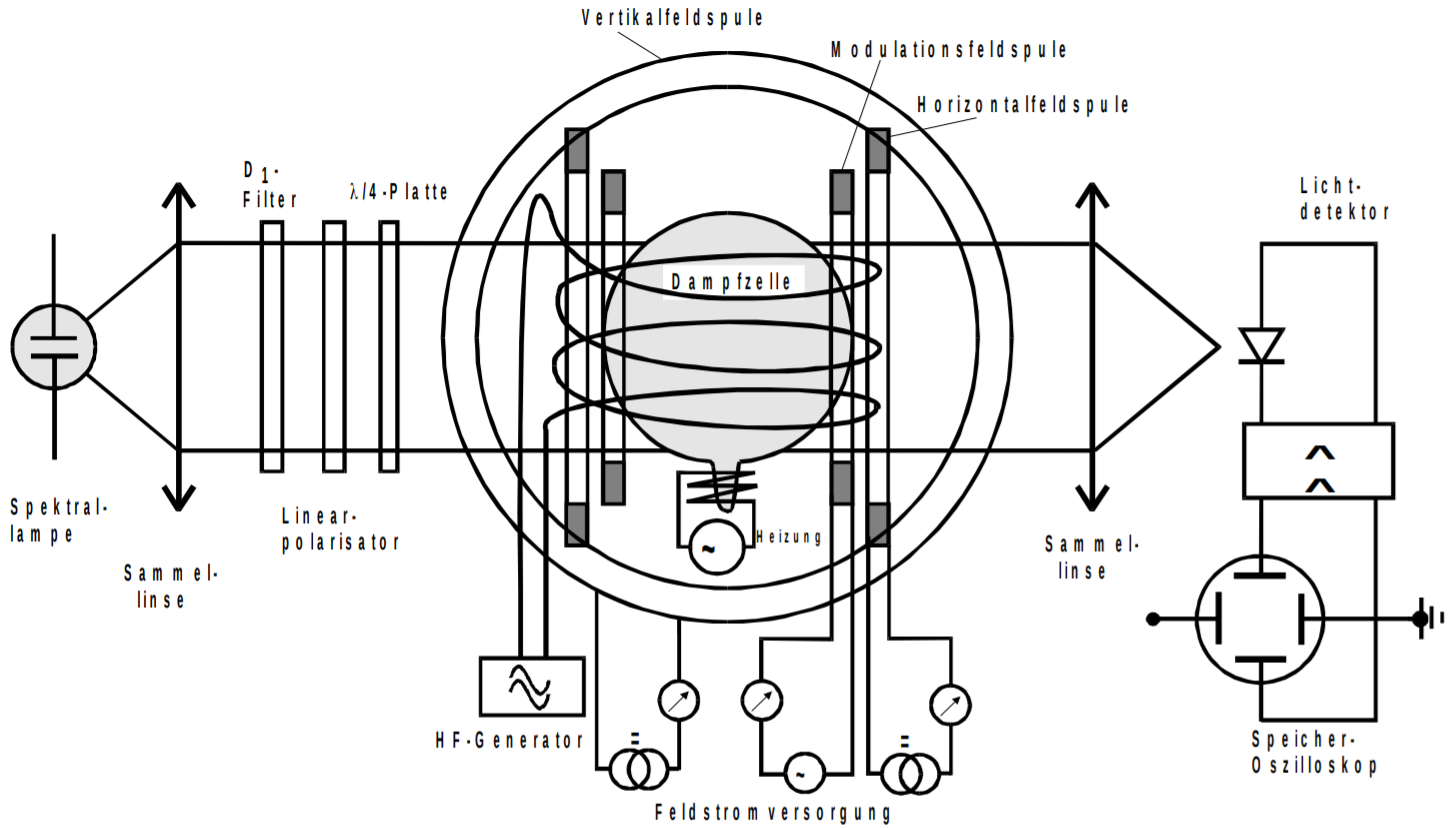
\includegraphics[width=0.9\textwidth]{Bilder/Aufbau}
  \caption{Schematische Darstellung des im Versuch genutzten Aufbaus \cite{anleitung}.}
  \label{aufbau}
\end{figure}
\subsection{Durchführung}
Zu Beginn des Versuchs muss das Erdmagnetfeld kompensiert werden. Hierzu wird der Tisch, auf welchem sich die Apparatur befindet zunächst mithilfe eines Kompasses nach der Horizontalkomponete des Erdmagnetfelds ausgerichtet. Nach Inbetriebnahme der Apparatur ist ein breiter Peak auf dem Oszilloskop zu sehen, welcher einen Einbruch der Transparenz der Rubidiumdampfzelle bei Abwesenheit eines Magnetfelds darstellt. Durch die Vertikal-Spulen ist es dann möglich die Breite des Peaks zu reduzieren und somit das Erdmagnetfeld zu kompensieren.\\
Anschließend kann die Untersuchung der Resonanzstellen der beiden Isotope beginnen. Hierzu wird die RF-Spule eingeschaltet und ihre Frequenz wird während der Untersuchung zwischen $100\, \si{\kilo\hertz}$ und $1\,\si{\mega\hertz}$ variiert. Es wird dann in $100\, \si{\kilo\hertz}$-Schritten die Feldstärke des RF-Feldes an den Resonanzstellen aufgezeichnet. Für höhere Frequenzen ist es in der Regel notwendig, ein zusätzliches horizontales Feld anzulegen.\\
Für den nächsten Abschnitt wird das RF-Spulenpaar zusätzlich an eine Rechtecksspannung mit einer Amplitude von $1\,\si{\volt}$ und einer Frequenz von $5\,\si{\hertz}$ angeschlossen. Das RF-Feld wird mit einem der Isotope in Resonanz geschaltet. Es werden sowohl das Signal der Rechtecksspannung als auch das der Photodiode auf dem Oszilloskop angezeigt. Die ansteigende Kurve des Signals wird daraufhin mit der Aufzeichnungsfunktion des Oszilloskops gespeichert. Dies wird an der abfallenden Flanke mit der Cursorfunktion die Zahl der Perioden der auftrendenden Schwingungen und die vergehende Zeit aufgezeichnet. Dieser Messprozess wird danach für das andere Isotop wiederholt.
\clearpage
